\addchap{Die Fakultät Informatik}

Der \emph{Andreas-Pfitzmann-Bau} (kurz APB, häufig auch einfach \glqq{}Fak\grqq{} genannt), das Gebäude welches die Fakultät Informatik beherbergt, wird in den nächsten 3 bis 5 Jahren dein zweites Zuhause sein.
Viele Lehrveranstaltungen und Übungen werden hier stattfinden. Mit zunehmender Semesterzahl wirst du immer weniger über den Campus gescheucht und immer mehr Veranstaltungen werden hier stattfinden.
Doch was hat dieser Bau eigentlich zu bieten außer einer Menge grüner Farbe und der Skulptur im Foyer?

\begin{figure}[h!]
\centering
\includegraphics[width=\linewidth]{img/panorama_fakultaet.jpg}
\caption*{\small \textit{Der Andreas-Pfitzmann-Bau von vorne -- Foto: Lucas Vogel}}
\end{figure}

Der wesentliche Unterschied zwischen diesem Gebäude und den anderen auf dem Campus ist, dass es rund um die Uhr geöffnet ist. Auch wenn nachts mal die Türen verschlossen sein sollten, wird euch der Nachtwächter gerne gegen Vorlage eures Studentenausweises die Tür öffnen und auf Wunsch auch einen der Seminarräume im Erdgeschoss aufschließen.
Auf die PC-Pools musst du nachts zwar verzichten, einer nächtlichen Lernorgie sollte aber trotzdem nichts im Wege stehen.

Außerdem können wir einen ziemlich schicken Außenbereich unser Eigen nennen. Dazu gehört ein Teich, viel Platz auf der Wiese zum Rumlümmeln und Außensteckdosen, die den Energiebedarf eines Informatikers problemlos decken. Da wir gerade beim Thema sind: Decken für diese Wiese stehen euch auch zur freien Verfügung und warten nur darauf, genutzt zu werden.
Von dem Teich aus kannst du außerdem das Rechenzentrum ("Lehmann-Zentrum") unserer Fakultät sehen. Vielleicht bekommst du ja die Chance und nehmt an einer der Führungen durch das Rechenzentrum teil, die zu verschiedenen Events angeboten werden.

% TODO: Mehr schreiben, um das Layout zu reparieren :eyes:

\pagebreak

\begin{figure}[t]
    \centering
    \includegraphics[width=\linewidth]{img/panorama_teich.jpg}
    \caption*{\small \textit{Der Andreas-Pfitzmann-Bau hinten raus -- Foto: Lucas Vogel}}
\end{figure}

Wie bereits erwähnt verfügt unsere Fakultät auch über mehrere PC-Pools, an denen du tagsüber arbeiten kannst. Die Computer verfügen über verschiedene Programme, die du für dein Studium brauchen wirst. Außerdem finden hier die vom FSR organisierten Programmierkurse statt.

Die Sitzgelegenheiten auf den Gängen aller Etagen bieten euch auch in der Prüfungsphase genügend Platz, um euch mit euren Lerngruppen auf die anstehenden Prüfungen vorzubereiten. Das \ascii{} wird dabei gerne euren Koffeinbedarf stillen.

% TODO: Change this to minisec? Adjust formatting for more :sparkle:? Same for Games Night!
\minisec{\textbf{ascii} – Das Café in der Fakultät}

Bereits seit 2007 existiert im Gebäude der Fakultät Informatik das \ascii{}, ein Café betrieben von Studenten für Studenten, Mitarbeiter und Besucher, kurzum: für jeden.
Das \ascii{} hat alles was ein richtiges Café so braucht: Kaffee, Kuchen, Bagels so wie alles was Nerds an der Fakultät so brauchen: Koffeinhaltige Kaltgetränke!
Zudem zählt das \ascii{} zu den wenigen Adressen auf dem Campus, wo man neben Club Mate auch Kolle Mate und Premium Cola erhält.
Hinter dem Tresen stehen Studierende, die gerne an einem Tag in der Woche noch ein paar Stündchen ihrer Freizeit zur Verfügung stellen.

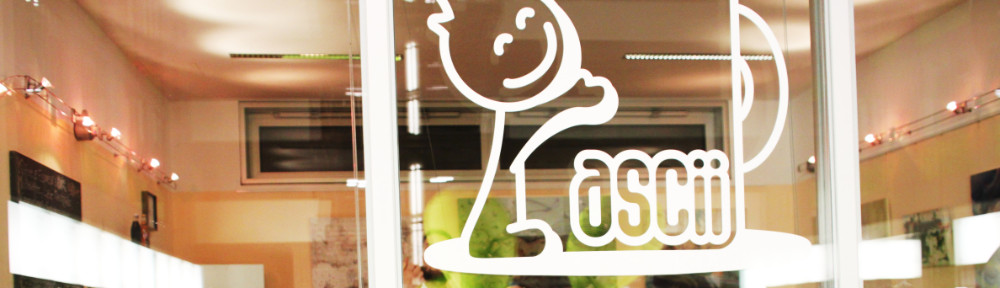
\includegraphics[width=\linewidth]{img/ascii.jpg}

Das \ascii{} wird von einem studentischen Verein betrieben und ist seit seiner Gründung eine zentrale Anlaufstelle für jede und jeden an der Fakultät.
Hier treffen sich Studierende, Mitarbeiter und Professoren um ihre Pausen zu verbringen,
zu arbeiten oder einfach ihren Koffeinhaushalt aufzufüllen.
Auf den gemütlichen Sofas kann man die Zeit wunderbar an sich vorbeistreichen lassen,
gemeinsam an Projekten arbeiten, lernen, programmieren oder einfach nur mit seinen Kommilitonen plaudern.
Du kennst noch niemanden an der Fakultät?
Du hast Fragen oder Gesprächsbedarf?
Wenn du ins \ascii{} kommst, wirst du schnell sehen, dass an dem Vorurteil, Nerds seien nicht sozial, absolut nichts dran ist.

Wenn du jetzt Lust bekommen hast, das \ascii{} zu besuchen oder sogar als Mitglied selbst mitzumachen, dann komm doch einfach mal vorbei und sag Hallo!

Weitere Hinweise findest du auf \link{https://www.ascii-dresden.de/}.

\textit{Wir öffnen in der Vorlesungszeit Montag bis Donnerstag von 9 bis 17 Uhr und Freitags von 9 bis 15 Uhr. Dazwischen sind wir aber auch häufig im Café anzutreffen.}
